\section{The geometry of graphs of functions}
In this chapter we want to study the geometry of curves: direction, speed, bending,
and twisting. This field of study is properly called \emph{differential geometry}.

In this section, we will discuss the geometry of the graphs of functions, and then over the next
few sections we will define and then talk about curves with more interesting and complex
properties.

\subsection{Slope and concavity}
Suppose $ \gamma $ is a function. If we walk along the graph of $ \gamma $, then
at each point $ (t, \gamma(t)) $ we have a measure of the direction that we are
pointing: we are pointing at an angle $ \arctan \gamma'(t) $ to the $ x$--axis.

\begin{figure}
  \centering
  \begin{tikzpicture}
    \begin{axis}[
        axis lines = center,
        xlabel = $ t $,
        ylabel = {$ y = \gamma(t) $},
        ticks = none
      ]
        \addplot[domain = 0:5, color = red, samples=100] {x^3 - x^2 - x - 1};
        \draw[->] (4,43) -- (4.33,56);
        \draw[dotted] (4,43) -- (4.33,43) -- (4.33,56);
        \draw[below] (4.165,43) node{$1$};
        \draw[right] (4.33,49.5) node{$\gamma'(t)$};
    \end{axis}
  \end{tikzpicture}
  \caption{Slope as a measure of direction.}
\end{figure}

We can essentially differentiate (if you pardon the pun) three different kinds of behaviour:
\begin{defn}
  Let $ \gamma $ be a function. Then:
  \begin{enumerate}
    \item If $ \gamma'(a) > 0 $, $ \gamma $ is said to be \emph{increasing} at $ a $.
    \item If $ \gamma'(a) = 0 $, $ \gamma $ is said to be \emph{stationary} at $ a $.
    \item If $ \gamma'(a) < 0 $, $ \gamma $ is said to be \emph{decreasing} at $ a $.
  \end{enumerate}
\end{defn}

However, this does not yet give us any information about the curvature of the graph
of $ \gamma $: the amount of `bending' taking place. Based on our studies so far, it
would make some sense to define curvature to be the rate of change of slope. Unfortunately,
it turns out that this definition is `incomplete' in some technical sense (we will
discuss this briefly when we talk about arc length). However, the second derivative $ \gamma'' $
is useful to us on its own merits; instead of curvature, we will call it \emph{concavity}.

\begin{defn}
  Let $ \gamma $ be a function. Then:
  \begin{enumerate}
    \item If $ \gamma''(a) > 0 $, $ \gamma $ is said to be \emph{concave up} (or \emph{convex}) at $ a $.
    \item If $ \gamma''(a) = 0 $, $ a $ is said to be an \emph{inflection point} of $ \gamma $.
    \item If $ \gamma''(a) < 0 $, $ \gamma $ is said to be \emph{concave down} (or simply \emph{concave}) at $ a $.
  \end{enumerate}

  If $ \gamma $ is concave up for all points $ a $ , then we call the function as a whole concave up (and likewise for concave down functions).
\end{defn}

\begin{figure}
  \centering
  \begin{tikzpicture}
    \begin{axis}[
      axis lines = center,
      ymax = 1.5, ymin = -1.5,
      xtick={-6.28, -4.7124, -3.14159, -1.5708, 1.5708, 3.14159, 4.7124, 6.28},
      xticklabels={$ -2\pi $, $ -\frac{3\pi}{2} $, $ -\pi $, $ -\frac{\pi}{2} $, $ \frac{\pi}{2} $, $ \pi $, $ \frac{3\pi}{2} $, $ 2\pi $},
      xlabel = $ x $,
      ylabel = $ y $
    ]
      \addplot[domain = -2*pi:2*pi, color = red, samples=100] {sin(deg(x))};
    \end{axis}
  \end{tikzpicture}
  \caption{The sine function.\label{fig:sine}}
\end{figure}

\begin{figure}
  \centering
  \begin{tikzpicture}
    \begin{axis}[
      axis lines = center,
      xlabel = $ x $,
      ylabel = {$ y $}
    ]
      \addplot[domain=-5:5, color=red, samples=200] {x^3};
      \addplot[domain=-10:10, color=blue, samples=200] {x^2};
    \end{axis}
  \end{tikzpicture}
  \caption{Graphs of $ x^n $ for odd $ n $ (red) and even $ n $ (blue).\label{fig:monomials}}
\end{figure}

\begin{exs}
  \begin{enumerate}
    \item The function $ x \mapsto x^2 $ is concave up everywhere, increasing for $ x > 0 $, and decreasing when $ x < 0 $.
    \item The function $ x \mapsto \sin x $ is concave down when $ (2n)\pi < x < (2n + 1)\pi $, and concave up when $ (2n + 1)\pi < x < (2n + 2)\pi $
          (for all integers $ n $). See figure \ref{fig:sine}
    \item The function $ x \mapsto x^3 $ has an inflection point at $ (0,0) $; to the left of this point, the function is concave
          down (the second derivative is negative) and to the right the function is concave up (the second derivative is positive).
    \item In general, functions of the form $ f(x) = x^n $ (for integer $ n \geq 0 $) have some fairly symmetric properties:
      \begin{itemize}
        \item If $ n $ is even, then $ y = f(x) $ is even around the $ x $-axis (i.e. $ f(-x) = f(x) $), has a minimum at $ (0,0) $, and
              tends to $ +\infty $ in both directions. (See the function graphed in blue in figure \ref{fig:monomials}.)
        \item If $ n $ is odd, then $ y = x^n $ is odd around the $ x $-axis (i.e. $ f(-x) = -f(x) $), has an inflection point at $ (0,0) $,
              and tends to $ -\infty $ towards the left and $ +\infty $ towards the right. (See the function graphed in red in the figure.)
      \end{itemize}
  \end{enumerate}
\end{exs}

\begin{figure}
  \centering
  \begin{tikzpicture}
    \begin{axis}[
      axis lines = center,
      xlabel = $ x $,
      ylabel = {$ y = f(x) $},
    ]
      \addplot[domain=-2:2, color=red, samples=200] {x^4 - 2*x^2 + 3};
    \end{axis}
  \end{tikzpicture}
  \caption{The graph of $ f(x) = x^4 - 2x^2 + 3 $.\label{fig:poly9}}
\end{figure}

\begin{ex}
  Consider the function defined by $ f(x) = x^4 - 2x^2 + 3 $ (figure \ref{fig:poly9}). Find the intervals on which $ f $
  is increasing or decreasing, find the intervals of concavity, and find any inflection points.

  \textit{Solution.} We have $ f'(x) = 4x^3 - 4x $. This function is zero at $ x \in \{-1, 0, 1\} $, and so (since the function
  is a positive cubic) $ f $ will be decreasing when $ x < -1 $, increasing when $ -1 < x < 0 $, decreasing when $ 0 < x < 1 $,
  and increasing when $ 1 < x $. We also have $ f''(x) = 12x^2 - 4 $ and so $ f''(x) = 0 $ when $ x = \pm \frac{1}{\sqrt{3}} $.
  Hence the function is concave up when $ x < -\frac{1}{\sqrt{3}} $, concave down when $ \abs{x} < \frac{1}{\sqrt{3}} $, and concave
  up when $ x > \frac{1}{\sqrt{3}} $. The inflection points will be $ x = \pm{1}{\sqrt{3}} $.
\end{ex}

\subsection{Continuity}
We have already mentioned continuity, when we discussed limits. We would like to call a
function continuous, intuitively, if its graph can be drawn without picking a pen up off
the page. This is insufficient: we cannot prove continuity of any function via this
definition! The precise definition of continuity was given by Bernard Bolzano in the early
1800s, and is one of the greatest historical breakthroughs in mathematics. His definition,
for us, is best stated in terms of limits:
\begin{defn}
  A function $ f $ is said to be \emph{continuous} at $ a $ if $ \lim_{x \to a} f(x) = f(a) $. If $ f $
  is continous for every $ a $ in its domain, the function as a whole is said to be continuous.
\end{defn}

It is perhaps unfortunate that the concepts of continuity and differentiability are not the same. The details of this
are studied in exercise \ref{exercise:contnotdif}.

\subsection{Arc length and curvature (optional)}
The second derivative measures the curvature of a graph based on our position as we walk along the $ x$--axis. A little thought
suggests that it might be more natural to measure the curvature based on our position as we walk along the graph itself: if we
take our graph and we slant it, for example, this doesn't change the visual `bendiness' of the graph but it does change the
relative position of the graph above the $ x$--axis and thus the values of $ \od[2]{y}{x} $ change.

Let us fix some point on our curve; as we walk along our curve, we measure the distance we travel from this point. After we stick
our graph into a coordinate system, this length (the \emph{arc length}) becomes a function of our position.

We will begin with a circle, which we might guess behaves very nicely. I will define the curvature $ \kappa $ of the circle to be the rate
of change of the angle $ \theta $ that our tangent line makes with the $ x$--axis as we walk along the curve, increasing $ s $:
in other words, $ \kappa = \od{\theta}{s} $.

\begin{figure}
  \centering
  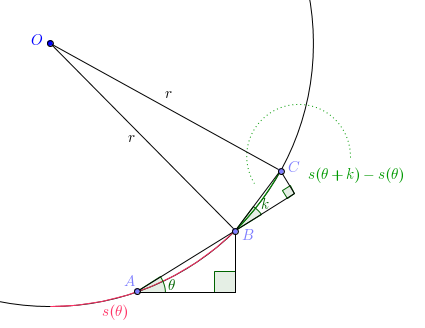
\includegraphics[width=0.6\textwidth]{curvaturecircle}
  \caption{Calculating the curvature of a circle.\label{fig:curvaturecircle}}
\end{figure}

Consider figure \ref{fig:curvaturecircle}. We are approximating a tangent line at $ B $ with the line $ AB $, and then
varying $ \theta $ by a small amount, $ k $. As our secant line $ AB $ approaches a tangent line, the angle at $ B $
between $ AB $ and the radius becomes a right angle. Similarly, the angle at $ C $ with the radius is a right angle for small $ k $. Thus the
angle at $ B $ in the triangle $ OBC $ is approximately $ \pi/2 - k $, and the angle at $ C $ is $ \pi/2 $; thus the angle at $ O $ is $ k $.

We therefore have that $ kr \approx s(\theta + k) - s(\theta) $, and so $ \od{s}{\theta} = r $; therefore $ \kappa = 1/r $.

If $ f $ is some arbitrary function, and we consider the graph $ y = f(x) $, we can calculate $ \od{\theta}{s} $ at each point (we will
do this calculation in a second). At each point, we can associate a circle with the same curvature; this circle is called the \emph{osculating
circle}, the radius $ r $ of the circle is the \emph{radius of curvature} of our graph at that point, and have will say that the \emph{curvature}
of the graph at the point $ x $ is $ \kappa = \od{\theta}{s} = 1/r $.

\begin{figure}
  \centering
  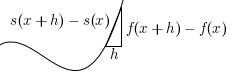
\includegraphics[width=0.3\textwidth]{curvaturefunc}
  \caption{Calculating the curvature of a function.\label{fig:curvaturefunc}}
\end{figure}

So now we will play the same game as above, but now with an arbitrary curve. Consider the function
in figure \ref{fig:curvaturefunc}; we will again denote the angle at $ x $ with the horizontal by $ \theta $.
As we increase $ x $ by $ h $, we increase $ s $ by $ s(x + h) - s(x) $. By definition of the
derivative, $ \od{s}{x} h \approx s(x + h) - s(x) = \sqrt{h^2 + (f(x+h) -f(x))^2} $; dividing through,
\begin{displaymath}
  \od{s}{x} \approx \sqrt{1 + \left(\frac{f(x + h) - f(x)}{h}\right)^2};
\end{displaymath}
and taking the limit $ h \to 0 $, we obtain
\begin{equation}
  \od{s}{x} = \sqrt{1 + \left(\od{y}{x}\right)^2} = \sqrt{1 + \tan^2 \theta} = \sec \theta.\label{eqn:sbyx}
\end{equation}

Furthermore, since $ \od{y}{x} = \tan \theta $ we have
\begin{displaymath}
  \od[2]{y}{x} = \od{}{x} \od{y}{x} = \od{}{x} \tan \theta = \od{\theta}{x} \sec^2 \theta
\end{displaymath}
and hence
\begin{equation}
  \od{x}{\theta} = \frac{\sec^2 \theta}{\left(\od[2]{y}{x}\right)}.\label{eqn:xbyth}
\end{equation}

Finally, by definition we have that the radius of curvature is (combining equations \ref{eqn:sbyx} and \ref{eqn:xbyth})
\begin{displaymath}
  r = \od{s}{\theta} = \od{s}{x} \od{x}{\theta} = \frac{\sec^3 \theta}{\left(\od[2]{y}{x}\right)};
\end{displaymath}
and the curvature is therefore (again by definition)
\begin{displaymath}
  \kappa(x) = \frac{1}{r} = \frac{\od[2]{y}{x}}{\sec^3\theta} = \frac{\od[2]{y}{x}}{\left(\sqrt{1 + \tan^2 \theta}\right)^3}
            = \frac{\od[2]{y}{x}}{\left(1 + \left(\od{y}{x}\right)^2\right)^{3/2}}.
\end{displaymath}


\subsection{Exercises and Problems}
\begin{enumerate}
  \item The following function is known as the \textit{logistic curve} and is used for population modelling. Find the intervals of
        concavity, and label any inflection points.
        \begin{center}
          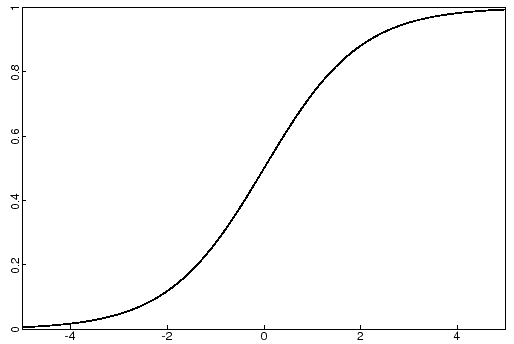
\includegraphics[width=0.4\textwidth]{logistic}
        \end{center}
  \item Find the second derivative of the following functions.
    \begin{enumerate}
      \item $ y = x^2 + x $
      \item $ f(x) = \sin x $
      \item $ g(x) = \cot(3x^2 + 5) $
      \item $ y = \frac{\sin mx}{x} $
      \item $ y = 4 \sin^2 x $
      \item $ y = \tan^2 (\sin \theta) $
      \item $ y = \tan \sqrt{1 - x} $
    \end{enumerate}
  \item Find the concavity of the function $ y = \frac{x^2 - 1}{x^2 + 1} $ at $ (0, -1) $.
  \item Find the intervals on which the following functions are increasing or decreasing, and
        find their intervals of concavity.
    \begin{enumerate}
      \item $ y = x^2 + 1 $
      \item $ y = 2x^3+ 3x^2 - 36x $
      \item $ G(x) = x - 4\sqrt{x} $
    \end{enumerate}
  \item The graph of $ y = f(x) $ (where $ f $ is a continuous function) is concave up for all $ x < 0 $, concave down for $ x > 0 $, and decreasing everywhere.
    \begin{enumerate}
      \item Sketch the graph of $ y = f(x) $.
      \item What can you say about $ f'(x) $ and $ f''(x) $ for $ x < 0 $ and $ x > 0 $?
      \item What about $ x = 0 $?
    \end{enumerate}
  \item Find a value of $ k $ such that the function $ F $ is continuous at $ x = -3 $, where
        \begin{displaymath}
          F(x) =
          \begin{cases}
            \frac{x^2 - 9}{x+3} & \text{if } x \neq -3,\\
            k                   & \text{if } x = -3.
          \end{cases}
        \end{displaymath}
  \item Show whether or not the function $ g $ is continuous at the three points $(2, g(2)) $, $ (3,g(3)) $, and  $(4,g(4)) $, where
        \begin{displaymath}
          g(x) =
          \begin{cases}
            2x-x^2              & \text{if } 0 \leq 2,\\
            2-x                 & \text{if } 2 < x \leq 3,\\
            x-4                 & \text{if } 3 < x \leq 4,\\
            \pi                 & \text{if } x \geq 4.
          \end{cases}
        \end{displaymath}
  \item Find all values of $ \alpha $ such that $ \Phi $ is continuous everywhere, where
        \begin{displaymath}
          \Phi(x) =
          \begin{cases}
            x+1                 & \text{if } x \leq \alpha, \\
            x^2                 & \text{if } x > \alpha.
          \end{cases}
        \end{displaymath}
  \item Sketch a function satisfying the given criteria.
    \begin{enumerate}
      \item
        \begin{itemize}
          \item Vertical asymptote at $ x = 0 $,
          \item $ f'(x) > 0 $ if $ x < -2 $,
          \item $ f'(x) < 0 $ if $ x > -2 $ ($ x \neq 0 $),
          \item $ f''(x) < 0 $ if $ x < 0 $, $ f''(x) > 0 $ if $ x > 0 $.
        \end{itemize}
      \item
        \begin{itemize}
          \item $ f'(0) = f'(2) = f'(4) = 0 $,
          \item $ f'(x) > 0 $ if $ x < 0 $ or $ 2 < x < 4 $,
          \item $ f'(x) < 0 $ if $ 0 < x < 2 $ or $ x > 4 $,
          \item $ f''(x) > 0 $ if $ 1 < x < 3 $,
          \item $ f''(x) < 0 $ if $ x < 1 $ or $ x > 3 $.
        \end{itemize}
    \end{enumerate}
  \item A curve is defined by the function $ f(x) = e^{-(x-k)^2} $. Find, in terms of $ k $, the $ x$-ordinates for which $ f''(x) = 0 $.
  \item It turns out that if a function $ f $ is differentiable at $ a $ then $ f $ is always continuous at $ a $, but the converse
        is not true: there exist continuous functions that are not differentiable. (In fact, there exist functions that are continuous
        everywhere but differentiable nowhere.) \label{exercise:contnotdif}
    \begin{enumerate}
      \item We will prove that differentiability of $ f $ at $ a $ implies continuity of $ f $ at $ a $; expand the following
            and use the limit laws to show that $ \lim_{x \to a} f(x) - f(a) = 0 $, carefully indicating where you use the existence
            of the derivative.
            \begin{displaymath}
              \left[\lim_{a \to x} f(x) - f(a)\right]\left[\lim_{a \to x} \frac{x - a}{x - a}\right]
            \end{displaymath}
      \item Give an example of a function which is continuous but not differentiable at some point.
    \end{enumerate}
  \item We will do some studies of convexity that may be familiar to students who have looked at the exercises on convexity
        in the algebra notes. We assume that all functions are continuous and differentiable everywhere for simplicity.
    \begin{enumerate}
      \item Show that if $ f $ is a convex function, and if $ P = (p,f(p)) $ and $ Q = (q,f(q)) $ are any two distinct points
            on the graph of $ f $, then for every point $ X = (x_1, x_2) $ on the line segment $ \overline{PQ} $, $ x_2 \geq f(x_1) $
            and equality is only obtained at the endpoints.
      \item Show that if $ f $ is a convex function, and if $ P = (p,f(P)) $ is a point on the graph of $ f $, then for every
            point $ (x_1,x_2) $ on the tangent line to $ f $ at $ P $, $ x_2 \leq f(x_1) $ and equality is only obtained at $ P $.
      \item Prove similar statements to (a) and (b) in the case that $ f $ is a concave function. [Hint: there is not much work
            involved, as long as one ponders the function $ -f $.]
    \end{enumerate}
  \item Scholarship 2010: Recall that the points of inflection of a curve are places where the second derivative
        changes sign. These are typically, \textbf{but not always}, points at which the second derivative is zero.

        Consider the curve $ y = \sqrt[3]{x} e^{-x^2} $.

        Write the second derivative in the form $ \od[2]{y}{x} = (ax^4 + bx^2 + x)e^{-x^2} x^{-5/3} $, and hence
        find the $ x$-ordinates of the points of inflection of the curve.
  \item Scholarship 2004: (You may wish to remind yourself how to perform long division of polynomials.) Consider the function
        \begin{displaymath}
          y = \frac{x^2}{1 + x^2},
        \end{displaymath}
        where $ -1 \leq x \leq 1 $. The gradient at the point $ x = 1 $ is $ \frac{1}{2} $.

        Hence show that there is a point with $ \frac{1}{4} \leq x \leq \frac{1}{2} $ where the gradient is also $ \frac{1}{2} $.
  \item Scholarship 2013: A function $ f $ is \textbf{even} if $ f(-x) = f(x) $ for all $ x $ in its domain, and \textbf{odd} if $ f(-x) = f(-x) $
        for all $ x $ in its domain.
    \begin{enumerate}
      \item Describe which polynomials are even, which are odd, and which are neither.
      \item Suppose that $ g $ is any even differentiable function defined for all real numbers (not necessarily a polynomial). Use the
            limit definition of the derivative to prove that $ g' $ is odd.
    \end{enumerate}
  \item Recall that we can define the derivative of $ f $ by $ \mathsf{D}f(x) = \lim_{y \to x} \frac{f(y) - f(x)}{y - x} $.
        We will generalise this, by writing $ \mathsf{SD}f(x) = \lim_{h \to 0} \frac{f(x + h) - f(x - h)}{2h} $.
        This is called the \emph{symmetric derivative} of $ f $.
    \begin{enumerate}
      \item In fact, we defined the derivative of $ f $ at $ x $ to be the unique $ f' $ such that $ f(x + h) \approx f(x) + hf'(x) $
            for small $ h $.\footnote{Then we defined the notation $ \varphi(x,h) \approx \psi(x,h) $ to mean that $ \varphi(x) = \psi(x) + \vartheta(h) $
            for some function $ \vartheta $ satisfying $ \vartheta(h)/h \to 0 $ as $ h \to 0 $.}

            Show that, for small $ h $, if $ f'(x) $ exists then $ f(x + h) - f(x - h) \approx 2hf'(h) $. Hence
            conclude that $ \mathsf{SD}f(x) = \mathsf{D}f(x) $ whenever the latter exists.
      \item The converse is not true: show that if we define $ f(x) = \abs{x} $, then $ \mathsf{SD} f(0) $ exists
            but $ \mathsf{D} f(0) $ does not.
      \item Define the \emph{second} symmetric derivative of $ f $ by
            \begin{displaymath}
              \mathsf{SD}^2 f(x) = \lim_{h \to 0} \frac{\frac{f(x + h) - f(x)}{h} - \frac{f(x) - f(x - h)}{h}}{h} = \lim_{h \to 0} \frac{f(x + h) - 2f(x) + f(x - h)}{h^2}.
            \end{displaymath}
            Show that whenever $ f''(x) = \mathsf{D}^2 f(x) $ exists then $ \mathsf{SD}^2 f(x) $ exists and has the same value; show that the converse
            does not hold (i.e. the existence of the second symmetric derivative does not imply the existence of the usual second derivative)
            by considering a suitable function, such as
            \begin{displaymath}
              \mathrm{sgn}(x) = \begin{cases} -1 & x < 0 \\ 0 & x = 0 \\ 1 & x > 0. \end{cases}
            \end{displaymath}
    \end{enumerate}
  \item One may recall from one of the L1 externals that we can recover a quadratic equation given a table of its values. Suppose
        we know that the following table gives points on the graph of $ f(x) = ax^2 + bx + c $.

        \begin{tabular}{c|c}
          $ x $ & $ f(x) $ \\
          $ 0 $ & $ -5 $ \\
          $ 1 $ & $ 2 $ \\
          $ 2 $ & $ 15 $
        \end{tabular}

        Define the \emph{discrete first and second derivatives} of $ f $ by $ \Delta f(x) = f(x + 1) - f(x) $ and $ \Delta^2 f(x) = \Delta f(x + 1) - \Delta f(x)  $.
        According to the god-given material in L1, we know that if $ f $ is a quadratic, then $ a = \frac{1}{2} \Delta^2 f(x) $ (for any choice of $ x $); in this
        example, we can fill in the table as follows:-

        \begin{tabular}{c|c|c|c}
          $ x $ & $ f(x) $ & $ \Delta f(x) $ & $ \Delta^2 f(x) $\\
          $ 1 $ & $ -5 $ & $ 7 $ & $ 6 $\\
          $ 2 $ & $ 2 $ & $ 13 $ & \\
          $ 3 $ & $ 15 $ &&
        \end{tabular}

        Hence $ a = 3 $. We can then write (since we know $ f $ is a quadratic) $ bx + c = f(x) - 3x^2 $, which tells us that $ b\cdot 1 + c = -8 $
        and $ b \cdot 2 + c = -10 $; hence $ b = (-10 - {}^{-}8)/1 = -2 $ and $ c = -6 $. \label{exercise:funtimeswithcalculus}

        \begin{enumerate}
          \item Justify the above steps. (Possible approach: $ hf''(x) \approx f'(x + h) - f'(x) $; set $ h = 1 $, and work out what fudge
                factor $ \vartheta(h) $ we have.)
          \item Develop a theory of discrete first and second derivatives. (Possible routes of study could include: finding a geometric
                meaning of the discrete derivatives; defining discrete $ n$th derivatives; studying the relationship between the discrete
                derivatives and the usual derivatives. You may also want to generalise my definition: instead of $ f(x + 1) - f(x) $,
                perhaps one might like to look at $ [f(x + k) - f(x)]/k $ (sans limit).)
        \end{enumerate}
  \item These problems relate to the optional section on curvature and arc length.
    \begin{enumerate}
      \item If $ y = f(x) $, formula \ref{eqn:sbyx} gives us the derivative of arc length with respect to distance
            along the $ x$-axis. What is the arc length along the graph of the function $ f(x) = \frac{1}{3}x^3 - x $
            between the vertical lines $ x = 0 $ and $ x = 5 $?
      \item Repeat (a) for the function $ g(x) = \ln \abs{\sec x} $.
      \item What is the curvature of a straight line?
      \item Calculate the curvature $ \kappa(x) $ of the function $ f(x) = x^2 $ at the points $ x = 0 $, $ x = 2 $, and $ x = 4 $.
            Draw the osculating circles at each of these points. What happens to $ \kappa(x) $ as $ x \to \infty $?
    \end{enumerate}
\end{enumerate}

\subsection{References}
A good introduction to the geometry of curves, and differential geometry in general, is \emph{Differential Geometry
of Curves and Surfaces} by Manfredo P. do Carmo.

For a discussion of the history of continuity, see J F Harper (2016): Defining continuity of
real functions of real variables, BSHM Bulletin: Journal of the British Society for the History
of Mathematics, DOI:10.1080/17498430.2015.1116053 (\url{http://homepages.ecs.vuw.ac.nz/~harper/harper16.pdf}).

Discrete derivatives (see exercise \ref{exercise:funtimeswithcalculus}) are useful when taking
derivatives numerically (say we have a table of numbers defining a function $ f $, but we don't
have a nice formula for it). The kinds of things one may want to search for in a library catalogue
are ``difference calculus'' or ``discrete calculus''.

\subsection{Homework}
\paragraph{Reading}
\begin{figure}
  \centering
  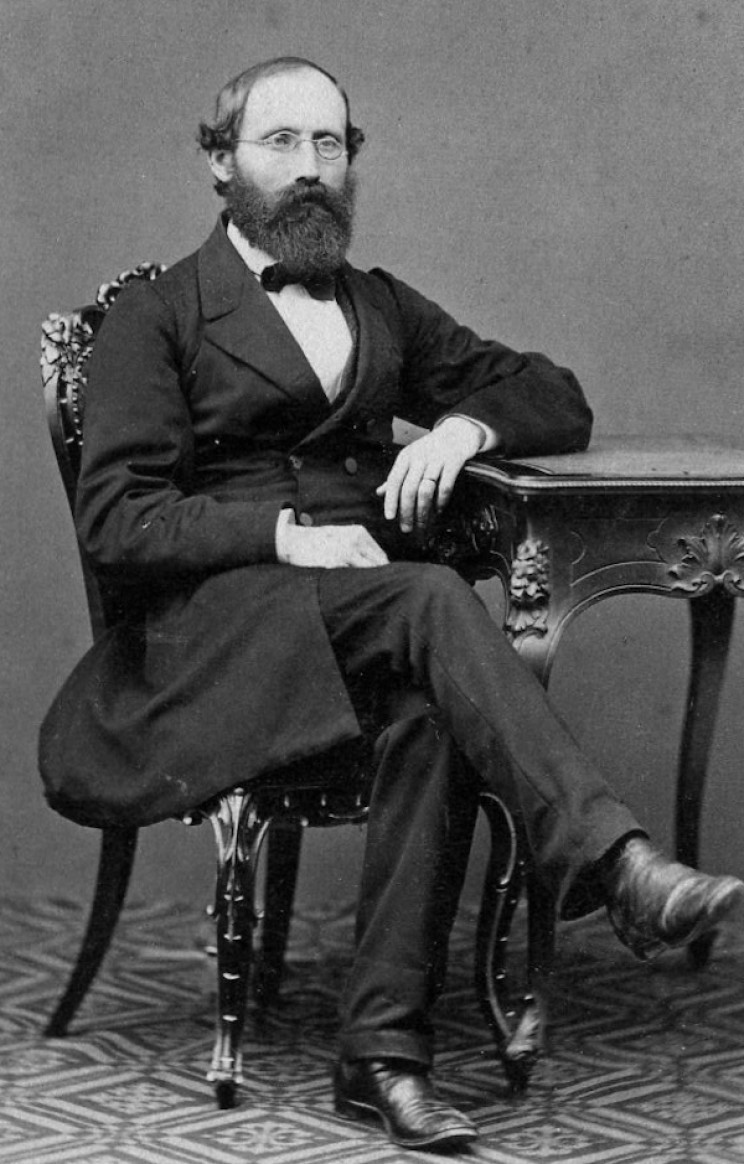
\includegraphics[width=0.2\textwidth]{riemann}
  \caption{Bernhard Riemann (public domain)}
\end{figure}
Bernhard Riemann (born September 17, 1826, Breselenz, Hanover [Germany] --- died July 20, 1866, Selasca, Italy) was a German mathematician whose profound and novel approaches to the study of geometry laid the mathematical foundation for Albert Einstein's theory of relativity. He also made important contributions to the theory of functions, complex analysis, and number theory.

Riemann was born into a poor Lutheran pastor's family, and all his life he was a shy and introverted person. He was fortunate to have a schoolteacher who recognized his rare mathematical ability and lent him advanced books to read, including Legendre's \textit{Number Theory} (1830). Riemann read the book in a week and then claimed to know it by heart. He went on to study mathematics at the University of Göttingen in 1846--47 and 1849--51 and at the University of Berlin (now the Humboldt University of Berlin) in 1847--49. He then gradually worked his way up the academic profession, through a succession of poorly paid jobs, until he became a full professor in 1859 and gained, for the first time in his life, a measure of financial security. However, in 1862, shortly after his marriage to Elise Koch, Riemann fell seriously ill with tuberculosis. Repeated trips to Italy failed to stem the progress of the disease, and he died in Italy in 1866.

Riemann's visits to Italy were important for the growth of modern mathematics there; Enrico Betti in particular took up the study of Riemannian ideas. Ill health prevented Riemann from publishing all his work, and some of his best was published only posthumously --- e.g., the first edition of Riemann's \textit{Gesammelte mathematische Werke} (1876; ``Collected Mathematical Works''), edited by Richard Dedekind and Heinrich Weber.

In 1854 Riemann presented his ideas on geometry for the official postdoctoral qualification at Göttingen; the elderly Gauss was an examiner and was greatly impressed. Riemann argued that the fundamental ingredients for geometry are a space of points (called today a manifold) and a way of measuring distances along curves in the space. He argued that the space need not be ordinary Euclidean space and that it could have any dimension (he even contemplated spaces of infinite dimension). Nor is it necessary that the surface be drawn in its entirety in three-dimensional space. A few years later this inspired the Italian mathematician Eugenio Beltrami to produce just such a description of non-Euclidean geometry, the first physically plausible alternative to Euclidean geometry. Riemann's ideas went further and turned out to provide the mathematical foundation for the four-dimensional geometry of space-time in Einstein's theory of general relativity. It seems that Riemann was led to these ideas partly by his dislike of the concept of action at a distance in contemporary physics and by his wish to endow space with the ability to transmit forces such as electromagnetism and gravitation.

\begin{flushright}
  Adapted from \textit{Bernhard Riemann} (by Jeremy John Gray) in the Encyclopaedia Britannica, \url{https://www.britannica.com/biography/Bernhard-Riemann}.
\end{flushright}

\paragraph{Problems}
\begin{enumerate}
  \item Explain, with sketches, the geometric meaning of the second derivative.
  \item Find the second derivative of the following functions.
    \begin{enumerate}
      \item $ f(x) = x^5 - 5x + 3 $
      \item $ f(x) = \frac{x^2}{x - 1} $
      \item $ f(x) = \sqrt{x} - \sqrt[4]{x} $
    \end{enumerate}
  \item Sketch a function satisfying the given criteria.
    \begin{enumerate}
      \item (hint: your result should be an odd function)
        \begin{itemize}
           \item $ f'(1) = f'(-1) = 0 $,
           \item $ f'(x) < 0 $ if $ \abs{x} < 1 $,
           \item $ f'(x) > 0 $ if $ 1 < \abs{x} < 2 $,
           \item $ f'(x) = -1 $ if $ \abs{x} > 2 $.
        \end{itemize}
      \item
        \begin{itemize}
          \item $ f'(x) < 0 $,
          \item $ f''(x) < 0 $.
        \end{itemize}
    \end{enumerate}
\end{enumerate}
